% BEGIN GENERATED:coverage_figure
% generator: cdrt.report 1 (coverage_figure)
% inputs: results/labs/lab7/attempt2/functional_records.jsonl f3606099382d; fixtures/out/parameters.json 2d3cdf7c84cb
% lock_root: 5027e2dd7806fc031b01e5880fcd83a8cca3381d7eb3cc3d5be6e4f1d233387c  campaign: campaign-002
% commit: 94766191d437ffb3b094db957e369b9e98784e51
\begin{figure}[pos=tbp]
\centering
% generator: cdrt.report 1 (figures/coverage.tex); lock_root: 5027e2dd7806fc031b01e5880fcd83a8cca3381d7eb3cc3d5be6e4f1d233387c; commit: 94766191d437ffb3b094db957e369b9e98784e51
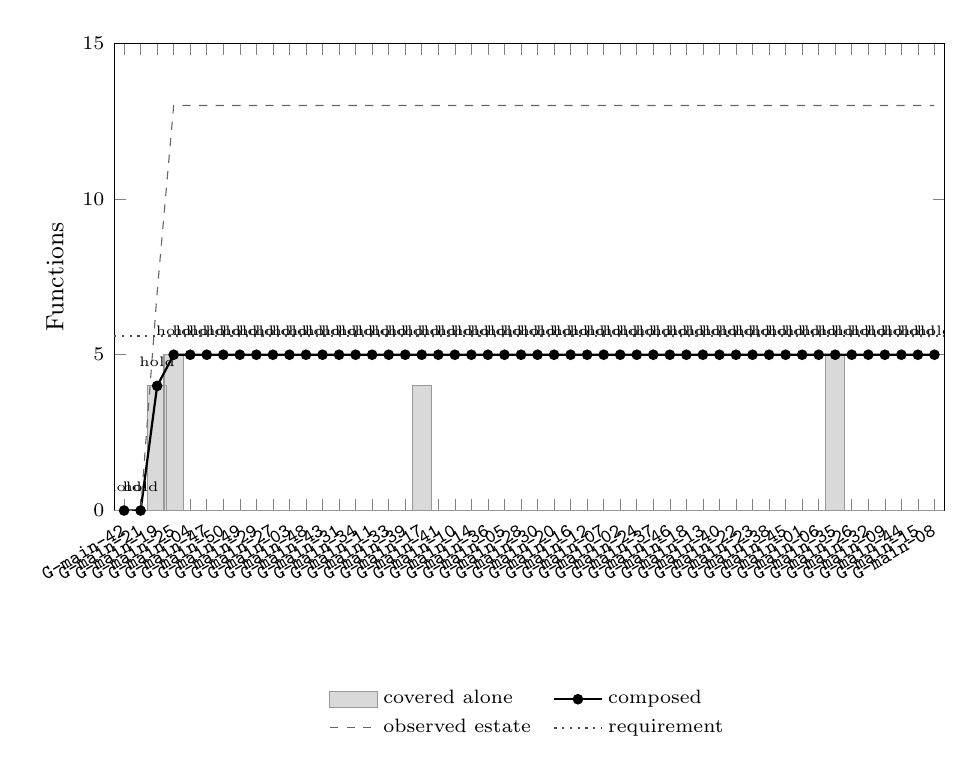
\begin{tikzpicture}
\begin{axis}[width=\columnwidth, height=0.62\columnwidth, ymin=0, ymax=15,
  xmin=0.4, xmax=50.6, xtick={1,2,3,4,5,6,7,8,9,10,11,12,13,14,15,16,17,18,19,20,21,22,23,24,25,26,27,28,29,30,31,32,33,34,35,36,37,38,39,40,41,42,43,44,45,46,47,48,49,50},
  xticklabels={{\texttt{G-main-42}},{\texttt{G-main-21}},{\texttt{G-main-19}},{\texttt{G-main-25}},{\texttt{G-main-04}},{\texttt{G-main-47}},{\texttt{G-main-50}},{\texttt{G-main-49}},{\texttt{G-main-29}},{\texttt{G-main-27}},{\texttt{G-main-03}},{\texttt{G-main-48}},{\texttt{G-main-43}},{\texttt{G-main-31}},{\texttt{G-main-34}},{\texttt{G-main-11}},{\texttt{G-main-33}},{\texttt{G-main-39}},{\texttt{G-main-17}},{\texttt{G-main-41}},{\texttt{G-main-10}},{\texttt{G-main-14}},{\texttt{G-main-36}},{\texttt{G-main-05}},{\texttt{G-main-28}},{\texttt{G-main-30}},{\texttt{G-main-20}},{\texttt{G-main-16}},{\texttt{G-main-12}},{\texttt{G-main-07}},{\texttt{G-main-02}},{\texttt{G-main-24}},{\texttt{G-main-37}},{\texttt{G-main-46}},{\texttt{G-main-18}},{\texttt{G-main-13}},{\texttt{G-main-40}},{\texttt{G-main-22}},{\texttt{G-main-23}},{\texttt{G-main-38}},{\texttt{G-main-45}},{\texttt{G-main-01}},{\texttt{G-main-06}},{\texttt{G-main-35}},{\texttt{G-main-26}},{\texttt{G-main-32}},{\texttt{G-main-09}},{\texttt{G-main-44}},{\texttt{G-main-15}},{\texttt{G-main-08}}},
  xticklabel style={font=\scriptsize, rotate=30, anchor=north east}, ylabel={Functions},
  tick label style={font=\scriptsize}, label style={font=\small},
  legend style={font=\scriptsize, at={(0.5,-0.36)}, anchor=north, draw=none, fill=none, legend columns=2,
    /tikz/every even column/.append style={column sep=6pt}}, legend cell align=left]
\addplot[ybar, bar width=7pt, fill=black!15, draw=black!40, area legend] coordinates {(1,0) (2,0) (3,4) (4,5) (5,0) (6,0) (7,0) (8,0) (9,0) (10,0) (11,0) (12,0) (13,0) (14,0) (15,0) (16,0) (17,0) (18,0) (19,4) (20,0) (21,0) (22,0) (23,0) (24,0) (25,0) (26,0) (27,0) (28,0) (29,0) (30,0) (31,0) (32,0) (33,0) (34,0) (35,0) (36,0) (37,0) (38,0) (39,0) (40,0) (41,0) (42,0) (43,0) (44,5) (45,0) (46,0) (47,0) (48,0) (49,0) (50,0)};
\addlegendentry{covered alone}
\addplot[thick, mark=*, mark size=1.5pt, black] coordinates {(1,0) (2,0) (3,4) (4,5) (5,5) (6,5) (7,5) (8,5) (9,5) (10,5) (11,5) (12,5) (13,5) (14,5) (15,5) (16,5) (17,5) (18,5) (19,5) (20,5) (21,5) (22,5) (23,5) (24,5) (25,5) (26,5) (27,5) (28,5) (29,5) (30,5) (31,5) (32,5) (33,5) (34,5) (35,5) (36,5) (37,5) (38,5) (39,5) (40,5) (41,5) (42,5) (43,5) (44,5) (45,5) (46,5) (47,5) (48,5) (49,5) (50,5)};
\addlegendentry{composed}
\addplot[dashed, black!60, mark=none] coordinates {(1,0) (2,0) (3,7) (4,13) (5,13) (6,13) (7,13) (8,13) (9,13) (10,13) (11,13) (12,13) (13,13) (14,13) (15,13) (16,13) (17,13) (18,13) (19,13) (20,13) (21,13) (22,13) (23,13) (24,13) (25,13) (26,13) (27,13) (28,13) (29,13) (30,13) (31,13) (32,13) (33,13) (34,13) (35,13) (36,13) (37,13) (38,13) (39,13) (40,13) (41,13) (42,13) (43,13) (44,13) (45,13) (46,13) (47,13) (48,13) (49,13) (50,13)};
\addlegendentry{observed estate}
\addplot[dotted, thick, black!70, domain=0.4:50.6] {5.6};
\addlegendentry{requirement}
\node[font=\tiny, anchor=south] at (axis cs:1,0.3) {hold};
\node[font=\tiny, anchor=south] at (axis cs:2,0.3) {hold};
\node[font=\tiny, anchor=south] at (axis cs:3,4.3) {hold};
\node[font=\tiny, anchor=south] at (axis cs:4,5.3) {hold};
\node[font=\tiny, anchor=south] at (axis cs:5,5.3) {hold};
\node[font=\tiny, anchor=south] at (axis cs:6,5.3) {hold};
\node[font=\tiny, anchor=south] at (axis cs:7,5.3) {hold};
\node[font=\tiny, anchor=south] at (axis cs:8,5.3) {hold};
\node[font=\tiny, anchor=south] at (axis cs:9,5.3) {hold};
\node[font=\tiny, anchor=south] at (axis cs:10,5.3) {hold};
\node[font=\tiny, anchor=south] at (axis cs:11,5.3) {hold};
\node[font=\tiny, anchor=south] at (axis cs:12,5.3) {hold};
\node[font=\tiny, anchor=south] at (axis cs:13,5.3) {hold};
\node[font=\tiny, anchor=south] at (axis cs:14,5.3) {hold};
\node[font=\tiny, anchor=south] at (axis cs:15,5.3) {hold};
\node[font=\tiny, anchor=south] at (axis cs:16,5.3) {hold};
\node[font=\tiny, anchor=south] at (axis cs:17,5.3) {hold};
\node[font=\tiny, anchor=south] at (axis cs:18,5.3) {hold};
\node[font=\tiny, anchor=south] at (axis cs:19,5.3) {hold};
\node[font=\tiny, anchor=south] at (axis cs:20,5.3) {hold};
\node[font=\tiny, anchor=south] at (axis cs:21,5.3) {hold};
\node[font=\tiny, anchor=south] at (axis cs:22,5.3) {hold};
\node[font=\tiny, anchor=south] at (axis cs:23,5.3) {hold};
\node[font=\tiny, anchor=south] at (axis cs:24,5.3) {hold};
\node[font=\tiny, anchor=south] at (axis cs:25,5.3) {hold};
\node[font=\tiny, anchor=south] at (axis cs:26,5.3) {hold};
\node[font=\tiny, anchor=south] at (axis cs:27,5.3) {hold};
\node[font=\tiny, anchor=south] at (axis cs:28,5.3) {hold};
\node[font=\tiny, anchor=south] at (axis cs:29,5.3) {hold};
\node[font=\tiny, anchor=south] at (axis cs:30,5.3) {hold};
\node[font=\tiny, anchor=south] at (axis cs:31,5.3) {hold};
\node[font=\tiny, anchor=south] at (axis cs:32,5.3) {hold};
\node[font=\tiny, anchor=south] at (axis cs:33,5.3) {hold};
\node[font=\tiny, anchor=south] at (axis cs:34,5.3) {hold};
\node[font=\tiny, anchor=south] at (axis cs:35,5.3) {hold};
\node[font=\tiny, anchor=south] at (axis cs:36,5.3) {hold};
\node[font=\tiny, anchor=south] at (axis cs:37,5.3) {hold};
\node[font=\tiny, anchor=south] at (axis cs:38,5.3) {hold};
\node[font=\tiny, anchor=south] at (axis cs:39,5.3) {hold};
\node[font=\tiny, anchor=south] at (axis cs:40,5.3) {hold};
\node[font=\tiny, anchor=south] at (axis cs:41,5.3) {hold};
\node[font=\tiny, anchor=south] at (axis cs:42,5.3) {hold};
\node[font=\tiny, anchor=south] at (axis cs:43,5.3) {hold};
\node[font=\tiny, anchor=south] at (axis cs:44,5.3) {hold};
\node[font=\tiny, anchor=south] at (axis cs:45,5.3) {hold};
\node[font=\tiny, anchor=south] at (axis cs:46,5.3) {hold};
\node[font=\tiny, anchor=south] at (axis cs:47,5.3) {hold};
\node[font=\tiny, anchor=south] at (axis cs:48,5.3) {hold};
\node[font=\tiny, anchor=south] at (axis cs:49,5.3) {hold};
\node[font=\tiny, anchor=south] at (axis cs:50,5.3) {hold};
\end{axis}
\end{tikzpicture}

\caption{Composed coverage as green decisions are admitted in capture order. Bars: release functions each decision covered on its own; solid line: release functions covered by all decisions admitted so far; dashed line: the size of the observed estate; dotted line: the requirement (\FixTauQ{} of \FixMq{}). The gateway reading after each admission is printed above. \CoverageSentence{}}
\label{fig:coverage}
\end{figure}
% END GENERATED:coverage_figure
